\documentclass[11pt]{article}
\usepackage{amsmath,amssymb,amsmath,amsthm,amsfonts}
\usepackage{latexsym,graphicx}
\usepackage{fullpage,color}
\usepackage{url,hyperref}
\usepackage{natbib}
\usepackage{graphicx,subfigure}
\usepackage{algorithm}
\usepackage{algorithmic}
\usepackage{listings}
\usepackage{xcolor}
\usepackage{color}

\numberwithin{equation}{section}

\pagestyle{plain}

\setlength{\oddsidemargin}{0in}
\setlength{\topmargin}{0in}
\setlength{\textwidth}{6.5in}
\setlength{\textheight}{8.5in}

\newtheorem{fact}{Fact}[section]
\newtheorem{question}{Question}[section]
\newtheorem{lemma}{Lemma}[section]
\newtheorem{theorem}[lemma]{Theorem}
\newtheorem{assumption}[lemma]{Assumption}
\newtheorem{corollary}[lemma]{Corollary}
\newtheorem{prop}[lemma]{Proposition}
\newtheorem{claim}{Claim}[section]
\newtheorem{remark}{Remark}[section]
\newtheorem{definition}{Definition}[section]
\newtheorem{prob}{Problem}[section]
\newtheorem{conjecture}{Conjecture}[section]
\newtheorem{property}{Property}[section]

\def\A{{\bf A}}
\def\a{{\bf a}}
\def\B{{\bf B}}
\def\bb{{\bf b}}
\def\C{{\bf C}}
\def\c{{\bf c}}
\def\D{{\bf D}}
\def\d{{\bf d}}
\def\E{{\bf E}}
\def\e{{\bf e}}
\def\F{{\bf F}}
\def\f{{\bf f}}
\def\g{{\bf g}}
\def\h{{\bf h}}
\def\G{{\bf G}}
\def\H{{\bf H}}
\def\I{{\bf I}}
\def\K{{\bf K}}
\def\k{{\bf k}}
\def\LL{{\bf L}}
\def\M{{\bf M}}
\def\m{{\bf m}}
\def\N{{\bf N}}
\def\n{{\bf n}}
\def\PP{{\bf P}}
\def\pp{{\bf p}}
\def\Q{{\bf Q}}
\def\q{{\bf q}}
\def\R{{\bf R}}
\def\rr{{\bf r}}
\def\S{{\bf S}}
\def\s{{\bf s}}
\def\T{{\bf T}}
\def\tt{{\bf t}}
\def\U{{\bf U}}
\def\u{{\bf u}}
\def\V{{\bf V}}
\def\v{{\bf v}}
\def\W{{\bf W}}
\def\w{{\bf w}}
\def\X{{\bf X}}
\def\x{{\bf x}}
\def\Y{{\bf Y}}
\def\y{{\bf y}}
\def\Z{{\bf Z}}
\def\z{{\bf z}}
\def\0{{\bf 0}}
\def\1{{\bf 1}}



\def\AM{{\mathcal A}}
\def\CM{{\mathcal C}}
\def\DM{{\mathcal D}}
\def\EM{{\mathcal E}}
\def\GM{{\mathcal G}}
\def\FM{{\mathcal F}}
\def\IM{{\mathcal I}}
\def\JM{{\mathcal J}}
\def\KM{{\mathcal K}}
\def\LM{{\mathcal L}}
\def\NM{{\mathcal N}}
\def\OM{{\mathcal O}}
\def\PM{{\mathcal P}}
\def\SM{{\mathcal S}}
\def\TM{{\mathcal T}}
\def\UM{{\mathcal U}}
\def\VM{{\mathcal V}}
\def\WM{{\mathcal W}}
\def\XM{{\mathcal X}}
\def\YM{{\mathcal Y}}
\def\RB{{\mathbb R}}
\def\RBmn{{\RB^{m\times n}}}
\def\EB{{\mathbb E}}
\def\PB{{\mathbb P}}

\def\TX{\tilde{\bf X}}
\def\TA{\tilde{\bf A}}
\def\tx{\tilde{\bf x}}
\def\ty{\tilde{\bf y}}
\def\TZ{\tilde{\bf Z}}
\def\tz{\tilde{\bf z}}
\def\hd{\hat{d}}
\def\HD{\hat{\bf D}}
\def\hx{\hat{\bf x}}
\def\nysA{{\tilde{\A}_c^{\textrm{nys}}}}

\def\alp{\mbox{\boldmath$\alpha$\unboldmath}}
\def\bet{\mbox{\boldmath$\beta$\unboldmath}}
\def\epsi{\mbox{\boldmath$\epsilon$\unboldmath}}
\def\etab{\mbox{\boldmath$\eta$\unboldmath}}
\def\ph{\mbox{\boldmath$\phi$\unboldmath}}
\def\pii{\mbox{\boldmath$\pi$\unboldmath}}
\def\Ph{\mbox{\boldmath$\Phi$\unboldmath}}
\def\Ps{\mbox{\boldmath$\Psi$\unboldmath}}
\def\ps{\mbox{\boldmath$\psi$\unboldmath}}
\def\tha{\mbox{\boldmath$\theta$\unboldmath}}
\def\Tha{\mbox{\boldmath$\Theta$\unboldmath}}
\def\muu{\mbox{\boldmath$\mu$\unboldmath}}
\def\Si{\mbox{\boldmath$\Sigma$\unboldmath}}
\def\si{\mbox{\boldmath$\sigma$\unboldmath}}
\def\Gam{\mbox{\boldmath$\Gamma$\unboldmath}}
\def\Lam{\mbox{\boldmath$\Lambda$\unboldmath}}
\def\De{\mbox{\boldmath$\Delta$\unboldmath}}
\def\Ome{\mbox{\boldmath$\Omega$\unboldmath}}
\def\Pii{\mbox{\boldmath$\Pi$\unboldmath}}
\def\varepsi{\mbox{\boldmath$\varepsilon$\unboldmath}}
\newcommand{\ti}[1]{\tilde{#1}}
\def\Ncal{\mathcal{N}}
\def\argmax{\mathop{\rm argmax}}
\def\argmin{\mathop{\rm argmin}}

\def\ALG{{\AM_{\textrm{col}}}}

\def\mean{\mathsf{mean}}
\def\std{\mathsf{std}}
\def\bias{\mathsf{bias}}
\def\var{\mathsf{var}}
\def\sgn{\mathsf{sgn}}
\def\tr{\mathsf{tr}}
\def\rk{\mathrm{rank}}
\def\nnz{\mathsf{nnz}}
\def\poly{\mathrm{poly}}
\def\diag{\mathsf{diag}}
\def\Diag{\mathsf{Diag}}
\def\const{\mathrm{Const}}
\def\st{\mathsf{s.t.}}
\def\vect{\mathsf{vec}}
\def\sech{\mathrm{sech}}
\def\sigmoid{\mathsf{sigmoid}}

\newcommand{\red}[1]{{\color{red}#1}}



\def\argmax{\mathop{\rm argmax}}
\def\argmin{\mathop{\rm argmin}}

\newenvironment{note}[1]{\medskip\noindent \textbf{#1:}}%
        {\medskip}


\newcommand{\etal}{{\em et al.}\ }
\newcommand{\assign}{\leftarrow}
\newcommand{\eps}{\epsilon}

\newcommand{\opt}{\textrm{\sc OPT}}
\newcommand{\script}[1]{\mathcal{#1}}
\newcommand{\ceil}[1]{\lceil #1 \rceil}
\newcommand{\floor}[1]{\lfloor #1 \rfloor}



\lstset{ %
extendedchars=false,            % Shutdown no-ASCII compatible
language=Python,                % choose the language of the code
xleftmargin=1em,
xrightmargin=1em,
basicstyle=\footnotesize,    % the size of the fonts that are used for the code
tabsize=3,                            % sets default tabsize to 3 spaces
numbers=left,                   % where to put the line-numbers
numberstyle=\tiny,              % the size of the fonts that are used for the line-numbers
stepnumber=1,                   % the step between two line-numbers. If it's 1 each line
                                % will be numbered
numbersep=5pt,                  % how far the line-numbers are from the code   %
keywordstyle=\color[rgb]{0,0,1},                % keywords
commentstyle=\color[rgb]{0.133,0.545,0.133},    % comments
stringstyle=\color[rgb]{0.627,0.126,0.941},      % strings
backgroundcolor=\color{white}, % choose the background color. You must add \usepackage{color}
showspaces=false,               % show spaces adding particular underscores
showstringspaces=false,         % underline spaces within strings
showtabs=false,                 % show tabs within strings adding particular underscores
frame=single,                 % adds a frame around the code
%captionpos=b,                   % sets the caption-position to bottom
breaklines=true,                % sets automatic line breaking
breakatwhitespace=false,        % sets if automatic breaks should only happen at whitespace
%title=\lstname,                 % show the filename of files included with \lstinputlisting;
%                                % also try caption instead of title
mathescape=true,escapechar=?    % escape to latex with ?..?
escapeinside={\%*}{*)},         % if you want to add a comment within your code
%columns=fixed,                  % nice spacing
%morestring=[m]',                % strings
%morekeywords={%,...},%          % if you want to add more keywords to the set
%    break,case,catch,continue,elseif,else,end,for,function,global,%
%    if,otherwise,persistent,return,switch,try,while,...},%
}


\begin{document}

%\setlength{\fboxrule}{.5mm}\setlength{\fboxsep}{1.2mm}
%\newlength{\boxlength}\setlength{\boxlength}{\textwidth}
%\addtolength{\boxlength}{-4mm}


\title{Logistic Regression}

\author{\textbf{Shusen Wang} \\ Stevens Institute of Technology}

%\date{ }

\maketitle

\begin{abstract}
	Logistic regression is the most popular linear and binary classifier.
	This article uses logistic regression as an example to demonstrate the whole procedure of machine learning.
	This article covers data processing, modeling, numerical optimization, prediction, evaluation metrics, and hyper-parameter tuning.
	Example Python implementations are provided. 
\end{abstract}

\section{Data}





Let $\x_1, \cdots , \x_n \in \RB^d$ be the training features and $y_1 , \cdots , y_n \in \{+1, -1\}$ be the training labels.
The data are store as a feature matrix $\X \in \RB^{n\times d}$ and vector $\y \in \{+1, -1\}^d$.
If the labels were in $\{0, 1\}$, instead of $\{-1, 1\}$, they must be converted to $\{-1, 1\}$.

For example, you can use the Diabetes dataset which has $768$ samples and $d=8$ features.
%We use $n=615$ samples for training and the rest for test.
Diabetes is a binary classification dataset with labels either $+1$ or $-1$.
The dataset can be downloaded from \url{https://www.csie.ntu.edu.tw/~cjlin/libsvmtools/datasets/}.


\subsection*{Feature scaling}

%Before introducing feature scaling, let us see a motivating example.
%Suppose a people's dataset has two features: $(\textrm{income}, \textrm{height})$.
%\begin{itemize}
%	\item 
%	Using US dollar as metric, people's income has a mean of 
%\end{itemize}

Here we study two kinds of feature scaling: min-max normalization and standardization.
Let us assume the data are unidimensional ($d=1$).
\begin{itemize}
	\item 
	Min-max normalization performs the transformation:
	\begin{equation*}
	x_i' \: = \: \frac{ x_i - \min (x) }{ \max (x) - \min (x) },
	\quad \textrm{for } i = 1 , \cdots , n.
	\end{equation*}
	The new features $\{ x_1', \cdots , x_n' \}$ are in the interval $[0, 1]$.
	\item 
	Standardization performs the transformation:
	\begin{equation*}
	x_i' \: = \: \frac{ x_i - \mean (x) }{ \std (x) },
	\quad \textrm{for } i = 1 , \cdots , n.
	\end{equation*}
	Here $\mean $ and $\std $ are the sample mean and sample standard deviation.
	The new features $\{ x_1', \cdots , x_n' \}$ have zero mean and unit variance.
\end{itemize}
Of course, real-world data are not unidimensional.
For $d > 1$, we can do feature scaling for every of the $d$ features independently.
For the feature matrix $\X \in \RB^{n\times d}$, the min-max normalization and standardization can be implemented using the following Python code.

\vspace{3mm}
\begin{lstlisting}
# Min-Max Normalization
import numpy

d = x.shape[1]
xmin = numpy.min(x, axis=0).reshape(1, d)
xmax = numpy.max(x, axis=0).reshape(1, d)
xnew = (x - xmin) / (xmax - xmin)
\end{lstlisting}
\vspace{3mm}

\vspace{3mm}
\begin{lstlisting}
# Standardization
import numpy

d = x.shape[1]
mu = numpy.mean(x, axis=0).reshape(1, d)
sig = numpy.std(x, axis=0).reshape(1, d)
xnew = (x - mu) / sig
\end{lstlisting}
\vspace{3mm}


Keep in mind that \textsf{xmin}, \textsf{xmax}, \textsf{mu}, and \textsf{sig} are all evaluated on the training set.
We must do the same trainsformation to both training and test features.
The following is what we actually do in practice.

\vspace{3mm}
\begin{lstlisting}
# Standardization
import numpy

# calculate mu and sig using the training set
d = x_train.shape[1]
mu = numpy.mean(x_train, axis=0).reshape(1, d)
sig = numpy.std(x_train, axis=0).reshape(1, d)

# transform the training features
x_train = (x_train - mu) / sig

# transform the test features
x_test = (x_test - mu) / sig
\end{lstlisting}
\vspace{3mm}




\section{Model}

Let $\x_1, \cdots , \x_n \in \RB^d$ be the training features and $y_1 , \cdots , y_n \in \{-1, 1\}$ be the training labels.
If the labels are in $\{0, 1\}$, instead of $\{-1, 1\}$, they must be converted to $\{-1, 1\}$.
The $\ell_2$-norm regularized logistic regression model is
\begin{equation} \label{eq:model}
\min_{\w \in \RB^d} \;
\Bigg\{  
Q (\w ; \X , \y ) \: \triangleq \:
\frac{1}{n}  \sum_{i=1}^n \log \Big( 1 + \exp \big( - y_i \w^T x_i \big) \Big) 
\, + \, \frac{\lambda}{2} \, \| \w \|_2^2 \Bigg\} .
\end{equation}
In \eqref{eq:model}, the average of the $n$ terms is the loss function, 
the term  $ \lambda \| \w \|_2^2$ is the regularization,
and $\lambda \geq 0$ is a tuning hyper-parameter.
The function $f(z) = \log (1 + e^{-z})$ is called logistic function, which is why the model is called logistic regression.


The following Python code computes the objective function $Q (\w ; \X , \y )$ for given $\w$, $\X$, $\y$, and parameter $\lambda$.


\vspace{3mm}
\begin{lstlisting}
# Calculate the objective function value
# Inputs:
#     w: d-by-1 matrix
#     x: n-by-d matrix
#     y: n-by-1 matrix
#     lam: scalar, the regularization parameter
# Return:
#     objective function value (scalar)
def objective(w, x, y, lam):
	n, d = x.shape
	yx = numpy.multiply(y, x) # n-by-d matrix
	yxw = numpy.dot(yx, w) # n-by-1 matrix
	vec1 = numpy.exp(-yxw) # n-by-1 matrix
	vec2 = numpy.log(1 + vec1) # n-by-1 matrix
	loss = numpy.mean(vec2) # scalar
	reg = lam / 2 * numpy.sum(w * w) # scalar
	return loss + reg
\end{lstlisting}
\vspace{3mm}



\subsection{Model derivation}


Logistic regression has two forms; \eqref{eq:model} is one of the two.
Here I derive both models using sigmoid function and cross-entropy function.
You can skip this subsection without affecting reading the rest of this article.


First, let us recall the definitions of sigmoid function and cross-entropy function.
The sigmoid function maps a real number (between $-\infty$ and $+\infty$) to a positive number in $(0, 1)$.
It is formally defined by 
\begin{equation*}
\sigmoid (z) 
\: \triangleq \: \frac{1}{ 1 + e^{-z} } .
\end{equation*}
The discrete cross-entropy function $H (\pp , \q )$ measures the distance between the two distributions, 
$\pp = [p_1, \cdots , p_k]^T$ and $\q= [q_1, \cdots , q_k]^T$.\footnote{Here, $\pp$ and $\q$ are $k$-dimensional vectors such that $p_1 , \cdots , p_k \geq 0$, $q_1 , \cdots , q_k \geq 0$, $p_1 + \cdots + p_k =1$, and $q_1 + \cdots + q_k =1$.}
It is defined by
\begin{equation*}
H (\pp, \q ) 
\: \triangleq \: - \sum_{i=1}^k p_i \log q_i .
\end{equation*}
Now we are ready to derive the logistic regression models.



\paragraph{Logistic regression (variant 1).}
The feature vector $\x \in \RB^d$ is the input to the model,
and the label is $y \in \{0, 1\}$ (different from the model \eqref{eq:model}).
The model has a trainable parameter vector $\w \in \RB^d$.
The prediction is made by the sigmoid function of $\x^T \w$:
\begin{equation*}
f (\x)
\: = \:
\sigmoid ( \x^T \w ) 
\: = \: \frac{1}{ 1 + \exp (-\x^T \w ) } .
\end{equation*}
The function $f( \x) \in (0, 1)$ is the predictor;
you can think of it as a dense layer with sigmoid activation function.
The function value is the probability that $\x$ is a positive sample;
therefore, $1 - f(\x)$ is the probability that $\x$ is negative sample.

Next, we use the label $y \in \{0, 1\}$ and the predictor $f (\x)$ to build a loss function.
Let $\pp \in \RB^{2}$ be 
\begin{equation*}
\pp \: = \: 
\left[
\begin{array}{c}
y \\
1-y \\
\end{array}
\right].
\end{equation*}
Define $\q \in \RB^2$ as
\begin{equation*}
\q \: = \: 
\left[
\begin{array}{c}
f (\x) \\
1 - f (\x) \\
\end{array}
\right] .
\end{equation*}
Obviously, both $\pp$ and $\q$ are probability distributions.
Note that $\q = \pp$ means perfect prediction;
so we hope $\q$ is as close to $\pp$ as possible, and thus define the loss function as
\begin{eqnarray*}
\textrm{Loss} (\x, y)
& = & H (\pp , \q )
\; = \; - \big( p_1 \log q_1 + p_2 \log q_2 \big) \\
& = & - \big[ y \log (f(\x)) + (1-y) \log (1-f(x))  \big] \\
& = & y \cdot \log \big[ 1 + \exp (-\x^T \w) \big]
+ (1-y) \x^T \w + (1- y) \cdot \log \big[ 1 + \exp (-\x^T \w)  \big] \\
& = & \log \big[ 1 + \exp (-\x^T \w) \big] + (1-y)  \x^T \w .
\end{eqnarray*}
Using all the $n$ training samples $(\x_1, y_1), \cdots , (\x_n, y_n)$, the final logistic regression model is
\begin{equation*}
\min_{\w \in \RB^d} \; \frac{1}{n} \sum_{i=1}^{n} \textrm{Loss} (\x_i, y_i ) ,
\end{equation*}
equivalently, 
\begin{equation} \label{eq:model1}
\min_{\w \in \RB^d} \; \frac{1}{n} \sum_{i=1}^{n} 
\Big\{ \log \big[ 1 + \exp (-\x^T \w) \big]  + (1-y)  \x^T \w \Big\} .
\end{equation}
We can add the $\ell_1$ or $\ell_2$-norm regularization to the objective function.


\paragraph{Logistic regression (variant 2).}
This variant is the model \eqref{eq:model} we study throughout.
Different from the other variant, here we require the label $y$ be either $+1$ or $-1$.
The model has a trainable parameter vector $\w \in \RB^d$.
We hope the linear function $\x^T \w$ is positive if $\x$ is a positive sample
and it is negative if $\x$ is a negative sample.
Equivalently, we hope $y \x^T \w$ is always positive.

Based on such intuiations, 
we do the transformation for the training samples:
\begin{equation*}
\tilde{\x} \: = \: y \x .
\end{equation*}
Therefore, we can always encourage  $\tilde{\x}^T \w$ to be positive.
The prediction is made by the sigmoid function of $\tilde{\x}^T \w$:
\begin{equation*}
f (\x, y)
\: = \:
\sigmoid ( \tilde{\x}^T \w ) 
\: = \:
\sigmoid ( y {\x}^T \w ) 
\: = \: \frac{1}{ 1 + \exp (-y \x^T \w ) } .
\end{equation*}
The predictor $f(\w)$ is the probability that $\tilde{\x}^T \w$ is positive;
thus we encourage $f(\x)$ as close to 1 as possible.
Let $\pp \in \RB^{2}$ be fixed as
\begin{equation*}
\pp \: = \: 
\left[
\begin{array}{c}
1 \\
0 \\
\end{array}
\right].
\end{equation*}
Define $\q \in \RB^2$ as
\begin{equation*}
\q \: = \: 
\left[
\begin{array}{c}
f (\x, y) \\
1 - f (\x, y) \\
\end{array}
\right] .
\end{equation*}
We define the loss function as
\begin{eqnarray*}
	\textrm{Loss} (\x, y)
	& = & H (\pp , \q )
	\; = \; - \big( p_1 \log q_1 + p_2 \log q_2 \big) 
	\; = \; - p_1 \log q_1 \\
	& = & - \log (f(\x, y)) 
	\; = \; \log \big[ 1 + \exp ( - y \x^T \w ) \big].
\end{eqnarray*}
Using all the $n$ training samples $(\x_1, y_1), \cdots , (\x_n, y_n)$, the final logistic regression model is
\begin{equation*}
\min_{\w \in \RB^d} \; \frac{1}{n} \sum_{i=1}^{n} \textrm{Loss} (\x_i, y_i ) .
\end{equation*}
If we further adding the $\ell_2$-norm regularization, then it becomes exactly \eqref{eq:model}.


\paragraph{Remark.}
Variant 1 is what we actually use in deep learning for binary classification, because the combination of sigmoid actiavation and binary cross-entropy is exactly the model \eqref{eq:model1}.
If we just do logistic regression itself, Variant 2 is easily to use than Variant 1.


\section{Training (Numerical Optimization)}


Given the training data $\X$ and $\y$, we seek to solve the optimization model \eqref{eq:model} to find minimum $\w^\star = \argmin_{\w} Q (\w ; \X , \y )$.
Logistic regression does not have close-formed solution, but we can use numerical optimization to arbitrarily approach $\w^\star$.
In this section, we introdue gradient descent (GD), stochastic gradient descent (SGD), accelerated SGD, and mini-batch SGD; all of them can solve the logistic regression model \eqref{eq:model}.



\subsection{Gradients} \label{sec:alg:grad}

Let $u = -y_i \w^T \x_i $, $v = e^u$, and $l_i = \log \big( 1 + \exp ( - y_i \w^T \x_i ) \big) = \log (1 + v)$.
We first compute the scalar derivatives:
\begin{equation*}
\frac{ \partial \, l_i }{\partial \, v}
\: = \: \frac{ \partial \, \log (1 + v) }{\partial \, v}
\: = \: \frac{1}{1+v} 
\: = \: \frac{1}{1+e^u}
\qquad \textrm{ and } \qquad
\frac{ \partial \, v }{\partial \, u}
\: = \: \frac{ \partial \, e^u }{\partial \, u}
\: = \: e^u  .
\end{equation*}
We then compute the derivative of scalar w.r.t.\ vector:
\begin{equation*}
\frac{ \partial \, u }{\partial \, \w }
\: = \: \frac{ \partial \, (-y_i \w^T \x_i) }{\partial \, \w }
\: = \: - y_i \x_i .
\end{equation*}
We finally apply the chain rule to get 
\begin{equation} \label{eq:grad1}
\frac{ \partial \, l_i }{\partial \, \w }
\: = \: \frac{ \partial \, u }{\partial \, \w } \, \frac{ \partial \, v }{\partial \, u } 
\, \frac{ \partial \, l_i }{\partial \, v} 
\: = \:  - y_i \x_i  \cdot e^u \cdot \frac{1}{1+e^u}
\: = \: \frac{ - y_i \x_i }{1+e^{-u}}
\: = \: \frac{ - y_i \x_i }{1+\exp({y_i \w^T \x_i})} .
\end{equation}
We can apply \eqref{eq:model} and \eqref{eq:grad1} to calculate the gradient of $Q$ (aka derivative of $Q (\w; \X , \y)$ w.r.t.\ $\w$):
\begin{equation*}\label{eq:grad2}
\nabla Q (\w) 
\: \triangleq \:
\frac{ \partial \, Q (\w ; \X , \y) }{\partial \, \w }
\: = \: \frac{1}{n} \sum_{i=1}^n \frac{ \partial \, l_i }{\partial \, \w } \, + \, \lambda \w 
\: = \: \frac{1}{n} \sum_{i=1}^n \frac{ -y_i \x_i }{1+\exp({y_i \w^T \x_i})} \, + \, \lambda \w  .
\end{equation*}



The following Python code calculate the full gradient of $Q $ at $\w$.
The code takes $\w$, $\X$, $\y$, and $\lambda$ and returns the full gradient.

\vspace{3mm}
\begin{lstlisting}
# Calculate the gradient
# Inputs:
#     w: d-by-1 matrix
#     x: n-by-d matrix
#     y: n-by-1 matrix
#     lam: scalar, the regularization parameter
# Return:
#     g: d-by-1 matrix, full gradient
def gradient(w, x, y, lam):
	n, d = x.shape
	yx = numpy.multiply(y, x) # n-by-d matrix
	yxw = numpy.dot(yx, w) # n-by-1 matrix
	vec1 = numpy.exp(yxw) # n-by-1 matrix
	vec2 = numpy.divide(yx, 1+vec1) # n-by-d matrix
	vec3 = -numpy.mean(vec2, axis=0).reshape(d, 1) # d-by-1 matrix
	g = vec3 + lam * w
	return g
\end{lstlisting}
\vspace{3mm}



\subsection{Gradient descent (GD)}

Let $\w_0 \in \RB^d$ be the initialization of $\w$;
for simple linear models, we typically use zero initialization.
The gradient of $Q$ at $\w_0$, denote 
\begin{equation*}
\nabla Q (\w_0)
\: = \: \frac{1}{n} \sum_{i=1}^n \frac{ - y_i \x_i }{1+\exp({y_i \w_0^T \x_i})} \, + \, \lambda \w_0 ,
\end{equation*} 
is the steepest ascent direction at $\w_0$.
In other words, if we want to increase the objective function $Q$ as much as possible, but we are only allow to move a tiny step away from $\w_0$, then we shall move along the gradient direction.
Since we want to minimize the objective function $Q$, we can move in the opposite direction of $\nabla Q (\w_0)$.
So we update $\w$ by:
\begin{equation*}
\w_1 \: \longleftarrow \:
\w_0 - \alpha \, \nabla Q (\w_0),
\end{equation*}
where $\alpha$ is the step size (aka learning rate) and needs tuning.
Then, we know $\w_1$, so we can calculate the gradient at $\w_1$ using \eqref{eq:grad2} to get 
\begin{equation*}
\nabla Q (\w_1)
\: = \: \frac{1}{n} \sum_{i=1}^n \frac{ - y_i \x_i }{1+\exp({y_i \w_1^T \x_i})} \, + \, \lambda \w_1 .
\end{equation*} 
We perform a similar update:
\begin{equation*}
\w_2 \: \longleftarrow \:
\w_1 - \alpha \, \nabla Q (\w_1).
\end{equation*}
We can repeat this procedure so on and so forth till the gradient $\nabla Q (\w_t)$ is close to zero or the objective function $Q (\w; \X, \y)$ stops decreasing.


\begin{figure}[!h]
	\centering
	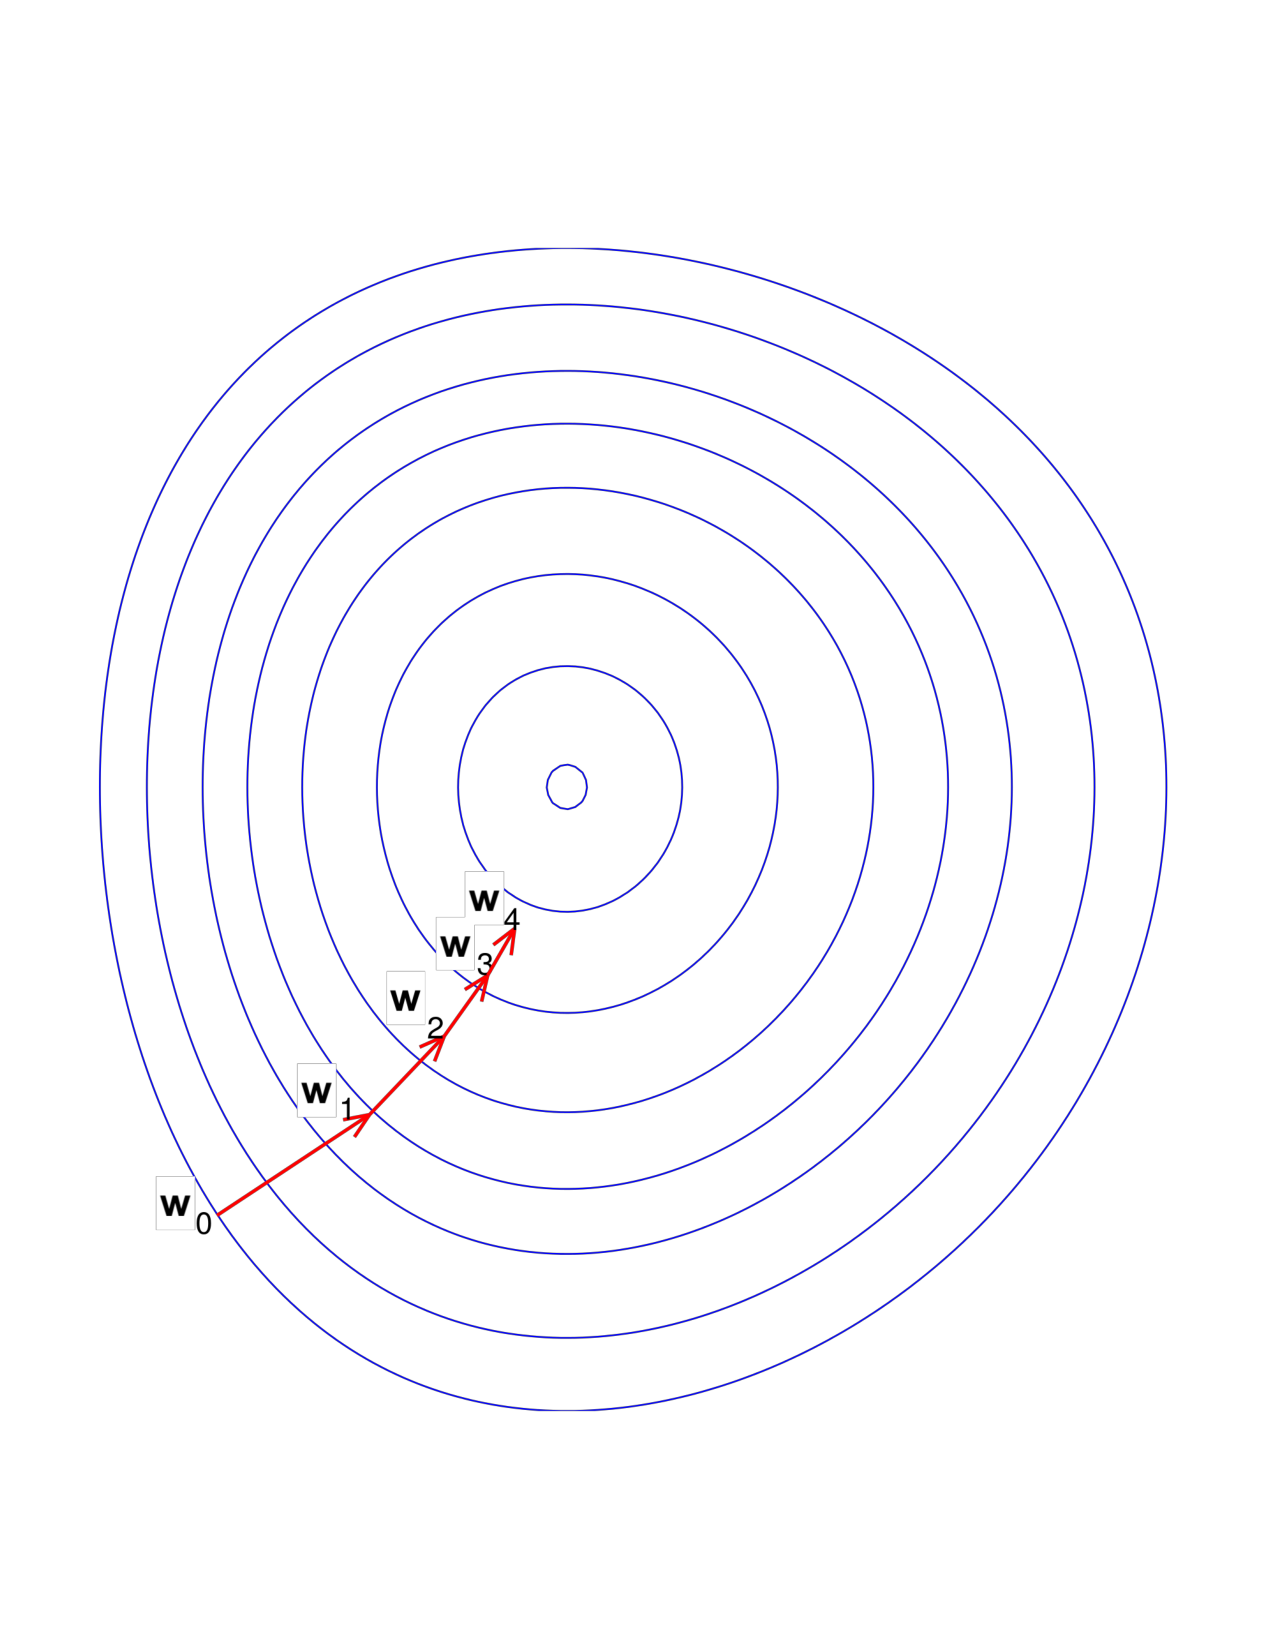
\includegraphics[width=0.5\linewidth]{figures/gradient_descent.pdf}
	\caption{Gradient descent.
		The figure is from Wikipedia.}
	\label{fig:gradient_descent}
\end{figure}


\paragraph{Algorithm.}
Gradient is illustrate in Figure~\ref{fig:gradient_descent} and formally described in the following.
\begin{enumerate}
	\item 
	Initialize $\w_0$, e.g., $\w_0 = \0$;
	\item
	For $t = 0, 1, 2, \cdots , T$, repeat the following steps:
	\begin{enumerate}
		\item 
		Use $\X$, $\y$, and $\w_t$ to calculate
		$\nabla Q (\w_t) \, = \, \frac{1}{n} \sum_{i=1}^n \frac{ - y_i \x_i }{1+\exp({y_i \w_t^T \x_i})} \, + \, \lambda \w_t $;
		\item
		Update $\w$ by
		$\w_{t+1} \longleftarrow \w_t - \alpha \nabla Q (\w_t)$;
	\end{enumerate}
	\item
	Output $\w_{T}$ as a (near) optimal solution to \eqref{eq:model}.
\end{enumerate}




The following Python code implements the full gradient algorithm.
User needs to specify the step size (aka learning rate) and maximal number of iterations (equal to epochs).
The default initialization of $\w$ is all-zero;
however, if the user happen to have a good estimate of $\w$, then a warm start (using the estimate to initialize $\w$) will make the convergence faster.

\vspace{3mm}
\begin{lstlisting}
# Gradient descent for solving logistic regression
# Inputs:
#     x: n-by-d matrix
#     y: n-by-1 matrix
#     lam: scalar, the regularization parameter
#     stepsize: scalar
#     max_iter: integer, the maximal iterations
#     w: d-by-1 matrix, initialization of w
# Return:
#     w: d-by-1 matrix, the solution
#     objvals: a record of each iteration's objective value
def grad_descent(x, y, lam, stepsize, max_iter=100, w=None):
	n, d = x.shape
	objvals = numpy.zeros(max_iter) # store the objective values
	if w is None:
		w = numpy.zeros((d, 1)) # zero initialization
	
	for t in range(max_iter):
		objval = objective(w, x, y, lam)
		objvals[t] = objval
		print('Objective value at t=' + str(t) + ' is ' + str(objval))
		g = gradient(w, x, y, lam)
		w -= stepsize * g
	
	return w, objvals
	
# example
lam = 1E-6
stepsize = 1.0
w, objvals_gd = grad_descent(x_train, y_train, lam, stepsize)
\end{lstlisting}
\vspace{3mm}



\paragraph{Time complexity.}
For the GD algorithm,
each iteration (one update of $\w$) goes one pass over all the $n$ training samples.
Thus one iteration equals one epoch. 
(Please refer to Section~\ref{sec:alg:terminologies} for the definition of terminologies.)
Each iteration of GD must compute a full gradient, which costs $\OM (nd)$ time.


Let $\w^\star = \argmin_{\w} Q (\w ; \X , \y)$ be the global minimum;
for $\lambda >0$, the global minimum is unique.
Theories guarantees that with $\lambda > 0$ and $\alpha$ properly set,
$\w_t$ converges to the global minimum $\w^\star$.
That is, for a sufficiently large $T$ (may be several hundreds or thousands), 
$\| \w_T - \w^\star \|_2$ is sufficiently small.




\subsection{Stochastic gradient descent (SGD)} \label{sec:alg:sgd}

In each iteration, the gradient descent algorithm computes $ \nabla Q (\w_t)$ according to \eqref{eq:grad2}.
The per-iteration time complexity is $\OM (n d)$.
In fact, computing the full gradient is unnecessary at all;
we can use stochastic gradient in lieu of the full gradient.



To derive stochastic gradient, let us express $Q $ as 
\begin{equation}\label{eq:sgrad1}
Q (\w; \X, \y) \: = \: \frac{1}{n} \sum_{i=1}^n Q_i(\w)  ,
\end{equation}
where
\begin{equation*}
Q_i (\w) \: = \: \log \Big( 1 + \exp \big( - y_i \w^T \x_i \big) \Big) + \frac{\lambda}{2} \|\w \|_2^2 .
\end{equation*}
Following Section~\ref{sec:alg:grad}, we can easily show that
\begin{equation} \label{eq:sgrad2}
\nabla Q_i (\w) \: \triangleq \:
\frac{ \partial \, Q_i (\w ) }{\partial \, \w }
\: = \:
\frac{ - y_i \x_i }{1+\exp({y_i \w^T \x_i})} \, + \, \lambda \w .
\end{equation}


\paragraph{Algorithm.}
Now we can present the SGD algorithm.
SGD is almost the same to gradient descent except for using $\nabla Q_i (\w_t)$ in lieu of $\nabla Q (\w_t)$.
SGD is formally described in the following.
\begin{enumerate}
	\item 
	Initialize $\w_0$, e.g., $\w_0 = \0$;
	\item
	For $t = 0, 1, 2, \cdots , T$, repeat the following steps:
	\begin{enumerate}
		\item
		Sample an index $i$ from $\{ 1 , 2, \cdots , n \}$ uniformly at random;
		\item 
		Use $\x_i$, $y_i$, and $\w_t$ to calculate
		$\nabla Q_i (\w_t) \, = \, \frac{-  y_i \x_i }{1+\exp({y_i \w_t^T \x_i})} \, + \, \lambda \w_t $;
		\item
		Update $\w$ by
		$\w_{t+1} \longleftarrow \w_t - \alpha \nabla Q_i (\w_t)$;
		\item
		Decrease the step size $\alpha$;
	\end{enumerate}
	\item
	Output $\w_{T}$ as a (near) optimal solution to \eqref{eq:model}.
\end{enumerate}


The following Python code implements SGD for solving logistic regression.
The function \textsf{stochastic\_objective\_gradient} calculates the value and gradient of $Q_i$ at $\w$.
User needs to specify the step size (aka learning rate) and maximal number of  epochs.
Difference from GD, the learning rate of SGD should be decreased after every epoch to guarantee convergence (see Line 32).

The actual implementation of SGD is slightly different from the above pseudo-code.
In each iteration of the pseudo-code, an index $i$ is randomly sampled from the set $\{ 1, \cdots , n \}$.
In practice, a better option is in each epoch, randomly shuffling the $n$ samples and then visiting the samples sequentially.




\vspace{3mm}
\begin{lstlisting}
# Calculate the objective Q_i and the gradient of Q_i
# Inputs:
#     w: d-by-1 matrix
#     xi: 1-by-d matrix
#     yi: scalar
#     lam: scalar, the regularization parameter
# Return:
#     obj: scalar, the objective Q_i
#     g: d-by-1 matrix, gradient of Q_i
def stochastic_objective_gradient(w, xi, yi, lam):
	d = xi.shape[0]
	yx = yi * xi # 1-by-d matrix
	yxw = float(numpy.dot(yx, w)) # scalar
	
	# calculate objective function Q_i
	loss = numpy.log(1 + numpy.exp(-yxw)) # scalar
	reg = lam / 2 * numpy.sum(w * w) # scalar
	obj = loss + reg
	
	# calculate stochastic gradient
	g_loss = -yx.T / (1 + numpy.exp(yxw)) # d-by-1 matrix
	g = g_loss + lam * w # d-by-1 matrix
	
	return obj, g
\end{lstlisting}
\vspace{3mm}



\vspace{3mm}
\begin{lstlisting}
# SGD for solving logistic regression
# Inputs:
#     x: n-by-d matrix
#     y: n-by-1 matrix
#     lam: scalar, the regularization parameter
#     stepsize: scalar
#     max_epoch: integer, the maximal epochs
#     w: d-by-1 matrix, initialization of w
# Return:
#     w: the solution
#     objvals: record of each iteration's objective value
def sgd(x, y, lam, stepsize, max_epoch=100, w=None):
	n, d = x.shape
	objvals = numpy.zeros(max_epoch) # store the objective values
	if w is None:
		w = numpy.zeros((d, 1)) # zero initialization
	
	for t in range(max_epoch):
		# randomly shuffle the samples
		rand_indices = numpy.random.permutation(n)
		x_rand = x[rand_indices, :]
		y_rand = y[rand_indices, :]
		
		objval = 0 # accumulate the objective values
		for i in range(n):
			xi = x_rand[i, :] # 1-by-d matrix
			yi = float(y_rand[i, :]) # scalar
			obj, g = stochastic_objective_gradient(w, xi, yi, lam)
			objval += obj
			w -= stepsize * g
		
		stepsize *= 0.9 # decrease step size; to be tuned
		objval /= n
		objvals[t] = objval
		print('Objective value at epoch t=' + str(t) + ' is ' + str(objval))
	
	return w, objvals
	
# example
lam = 1E-6
stepsize = 0.1
w, objvals_sgd = sgd(x_train, y_train, lam, stepsize)
\end{lstlisting}
\vspace{3mm}



\paragraph{Time complexity.}
Each iteration of SGD merely uses one training sample $(\x_i, y_i)$ and costs $\OM (d)$ time.
The per-iteration time complexity of SGD is tremendously smaller than GD, 
but SGD takes much more iterations to converge.
For SGD, one epoch equals to $n$ iterations.
Measured by epochs, SGD's convergence is faster than GD.


\paragraph{Theory.}
Why does SGD work?
It is because stochastic gradient is an unbiased estimate of the full gradient:
\begin{eqnarray*}
\EB_{i} \big[ \nabla Q_i (\w ) \big]
\: = \: \sum_{j=1}^n \frac{1}{n}  \nabla Q_j (\w ) 
\: = \: \nabla Q (\w) .
\end{eqnarray*}
Here, the expectation is taken w.r.t.\ the random index $i$.
Since $i$ can be any of $1, 2, \cdots , n$ with probability $\frac{1}{n}$,
the expectation can be written as a summation, by which the former identity follows.
The latter identity follows from \eqref{eq:sgrad1}.







\subsection{Mini-batch SGD}


Mini-batch SGD (MB-SGD) is straightforward extension of SGD.
In the previous subsection, we defined the function
\begin{equation*}
Q_i (\w) \: = \: \log \Big( 1 + \exp \big( - y_i \w^T \x_i \big) \Big) + \frac{\lambda}{2} \|\w \|_2^2 
\end{equation*}
and derived its gradient at $\w$, $\nabla Q_i (\w)$, as defined in \eqref{eq:sgrad2}.
We showed $\nabla Q_i (\w)$ is an unbiased estimate of $\nabla Q (\w)$, provided that $i$ is sampled uniformly at random:
\begin{equation*}
\EB_{i\sim p} \big[ \nabla Q_i (\w) \big]
\: = \: \nabla Q (\w) ,
\qquad \textrm{ where } p(i) = \tfrac{1}{n} \textrm{ for } i \in \{1, \cdots , n \} .
\end{equation*}
Let $\IM$ be a random set with cardinality $b$;
to be specific, every element in $\IM$ is uniformly sampled from $\{1, \cdots , n \}$ without replacement.
Define the function
\begin{equation*}
Q_{\IM} (\w) \: = \: \frac{1}{b} \sum_{i \in \IM} \log \Big( 1 + \exp \big( - y_i \w^T \x_i \big) \Big) + \frac{\lambda}{2} \|\w \|_2^2 .
\end{equation*}
Its gradient at $\w$ is
\begin{equation} \label{eq:mb_grad}
\nabla Q_{\IM} (\w) \: \triangleq \:
\frac{ \partial \, Q_{\IM} (\w ) }{\partial \, \w }
\: = \:
\frac{1}{b} \sum_{i \in \IM}  \frac{ - y_i \x_i }{1+\exp({y_i \w^T \x_i})} \, + \, \lambda \w .
\end{equation}
Mini-batch SGD uses $\nabla Q_{\IM} (\w)$, instead of $\nabla Q_i (\w)$, to update $\w$.
SGD is a special case of mini-batch SGD with $b=1$.
We can similarly prove that
\begin{equation*}
\EB_{\IM } \big[ \nabla Q_{\IM} (\w) \big]
\: = \: \nabla Q (\w) ,
\end{equation*}
where the expectation is taken w.r.t.\ the random set $\IM$.


\paragraph{Algorithm.}
The MB-SGD algorithm is almost the same as SGD except for using $\nabla Q_{\IM} (\w_t)$ instead of $\nabla Q_i (\w_t)$.
MB-SGD is formally described in the following.
\begin{enumerate}
	\item 
	Initialize $\w_0$, e.g., $\w_0 = \0$;
	\item
	For $t = 0, 1, 2, \cdots , T$, repeat the following steps:
	\begin{enumerate}
		\item
		Uniformly sample $b$ indices from $\{ 1 , 2, \cdots , n \}$ without replacement as a set $\IM$;
		\item 
		Use $\{ (\x_i, y_i) \}_{i \in \IM}$ and $\w_t$ to calculate
		$\nabla Q_{\IM} (\w_t) \, = \, \frac{1}{b} \sum_{i \in \IM} \frac{-  y_i \x_i }{1+\exp({y_i \w_t^T \x_i})} \, + \, \lambda \w_t $;
		\item
		Update $\w$ by
		$\w_{t+1} \longleftarrow \w_t - \alpha \nabla Q_{\IM} (\w_t)$;
		\item
		Decrease the step size $\alpha$;
	\end{enumerate}
	\item
	Output $\w_{T}$ as a (near) optimal solution to \eqref{eq:model}.
\end{enumerate}
MB-SGD can be implemented in Python by slightly changing the code of SGD.




MB-SGD has almost the same convergence properties as SGD.
In practice, mini-batch is a default setting for SGD and other stochastic optimization algorithms, e.g., Adagrad, RMSProp, etc.
When mentioning SGD, Adagrad, and RMSProp in practical papers and projects, people typically mean the mini-batch variants.




\subsection{Accelerated GD and SGD}

The convergence of GD and SGD critically depends on the {\bf condition number} of the problem.
For ill-conditioned problems (i.e., $\kappa$ is large), as illustrated in Figure~\ref{fig:sgd},
the convergence of SGD is extremely slow.
The steepest descending direction is not necessarily the best descending direction;
in fact, following the steepest descending direction, the path will be zig-zag.





\begin{figure}[!h]
	\centering
	\subfigure[SGD]{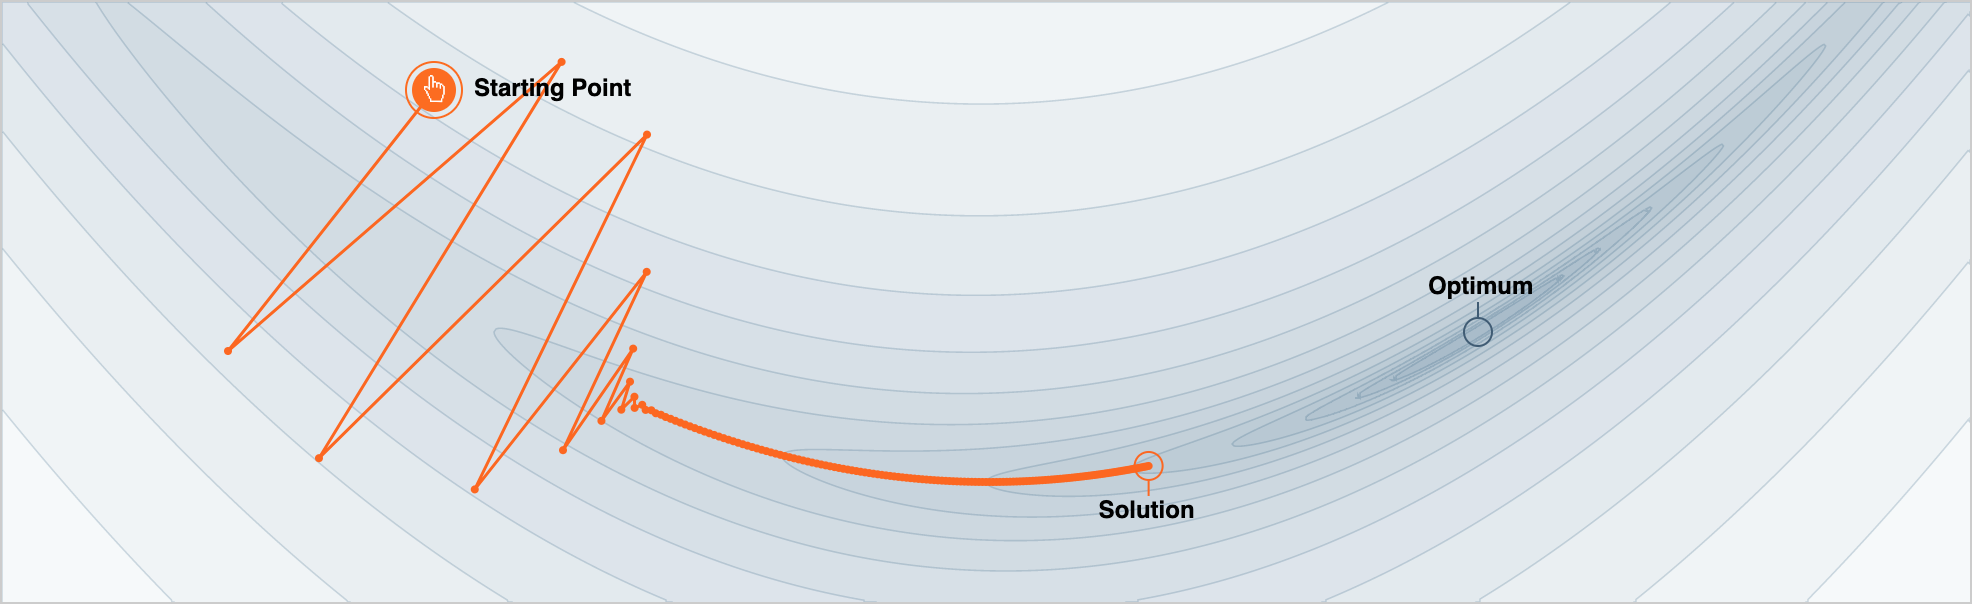
\includegraphics[width=0.8\linewidth]{figures/sgd1.png}}
	\subfigure[SGD with momentum]{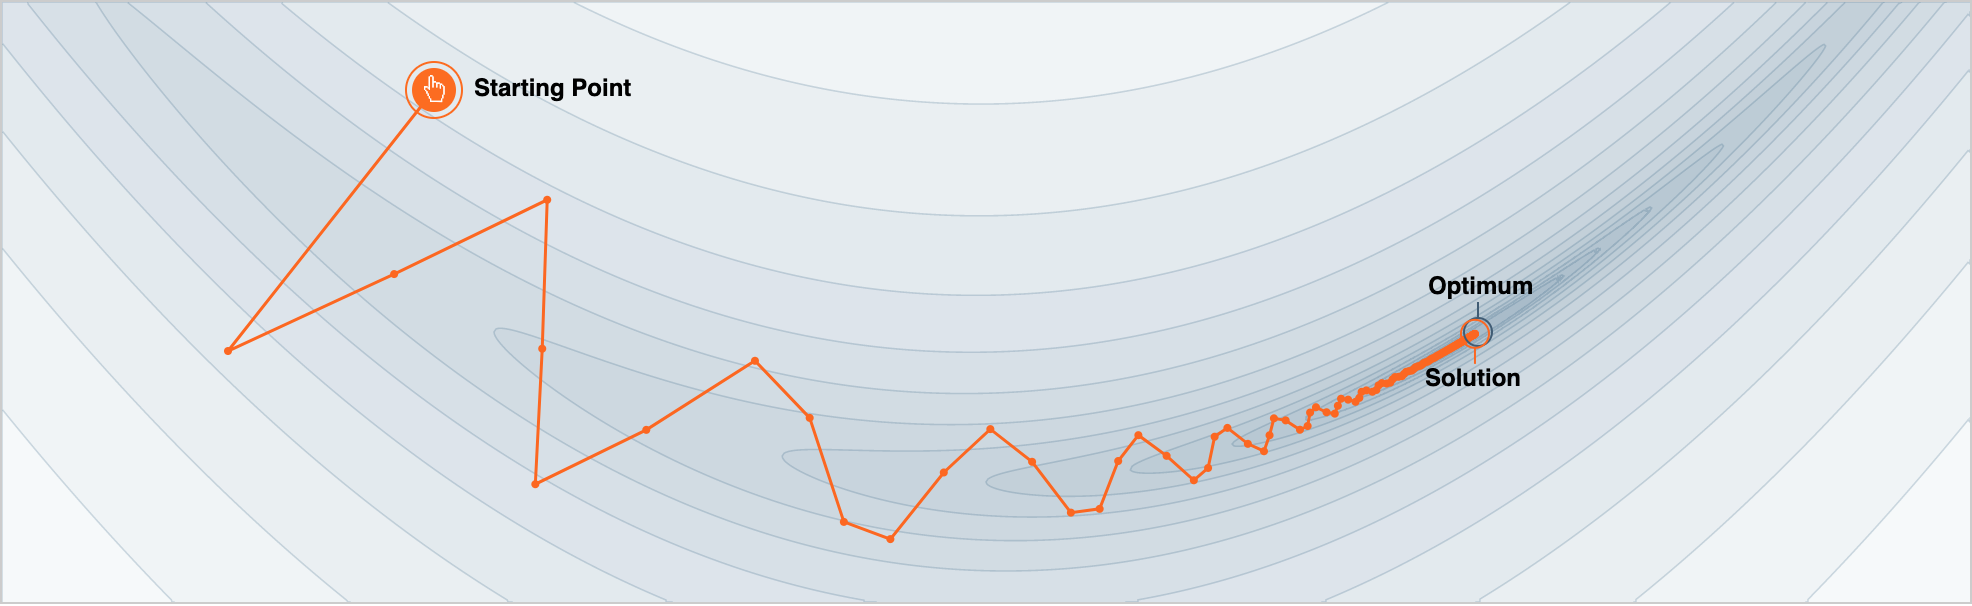
\includegraphics[width=0.8\linewidth]{figures/sgd2.png}}
	\caption{SGD and SGD with momentum. 
		The figures are from \url{https://distill.pub/2017/momentum/}.}
	\label{fig:sgd}
\end{figure}


Accelerated gradient algorithm uses the historical descending directions to correct the current descending direction to circumvent the zig-zag like path.
Accelerated gradient algorithm can significantly speed up computation, especially for ill-conditioned problems.
There are many accelerated algorithms based on the same idea.
Figure~\ref{fig:sgd} shows the advantage of SGD without momentum.


Here we describe only SGD with momentum; GD and MB-SGD with momentum are analogous.
SGD with momentum maintains a momentum vector $\z_t$
and take the momentum direction instead of the stochastic gradient direction.
Here is the update rule:
\begin{eqnarray*}
\z_{t+1} & \longleftarrow & \beta \z_t + \nabla Q_i (\w_t ), \\
\w_{t+1} & \longleftarrow & \w_t - \alpha \z_{t+1} .
\end{eqnarray*}
In the update rule,
$\alpha > 0$ and $\beta \in (0, 1)$ are two hyper-parameters affecting the convergence rate.
If the condition number is large (which is bad), $\beta$ should be set large, e.g., $\beta = 0.99$.
For SGD with momentum, we can safely use fixed $\alpha$;
differently, for SGD, $\alpha$ must decay after every epoch to guarantee convergence.
.







\subsection{Fairly comparing algorithms}

The following code compares GD and SGD by plotting their objective function values against epochs.
The output of the code is Figure~\ref{fig:compare_gd_sgd}.
Besides the plot of objective against epochs,
you can also plot the training accuracy against epochs or the validation accuracy against epochs.
The followings are typical pitfalls:
\begin{itemize}
	\item 
	Plot of objective or accuracy against runtime.
	It is fine if the algorithms are implemented in Fortran, C, or C++.
	However, if your implementation is Python, MATLAB, or R, such a comparison is very unfair to SGD, as for-loop  in Python, MATLAB, and R is very slow.
	\item
	Plot of objective or accuracy against iterations.
	This is a very bad idea for comparing different algorithms.
	For example, in Figure~\ref{fig:compare_gd_sgd}, if you change $x$-axis to iterations, GD takes around 50 iterations to converge, while SGD takes around 20,000 iterations;
	however, such a comparison does not make any sense.
\end{itemize}
In sum, when you compare the convergence of two optimization algorithms, the most straightforward approach is plotting objective or accuracy against epochs.



\vspace{3mm}
\begin{lstlisting}
import matplotlib.pyplot as plt
%matplotlib inline

fig = plt.figure(figsize=(6, 4))

epochs_gd = range(len(objvals_gd))
epochs_sgd = range(len(objvals_sgd))

line0, = plt.plot(epochs_gd, objvals_gd, '--b', LineWidth=4)
line1, = plt.plot(epochs_sgd, objvals_sgd, '-r', LineWidth=2)
plt.xlabel('Epochs', FontSize=20)
plt.ylabel('Objective Value', FontSize=20)
plt.xticks(FontSize=16)
plt.yticks(FontSize=16)
plt.legend([line0, line1], ['GD', 'SGD'], fontsize=20)
plt.tight_layout()
plt.show()
fig.savefig('compare_gd_sgd.pdf', format='pdf', dpi=1200)
\end{lstlisting}
\vspace{3mm}




\begin{figure}[!h]
	\centering
	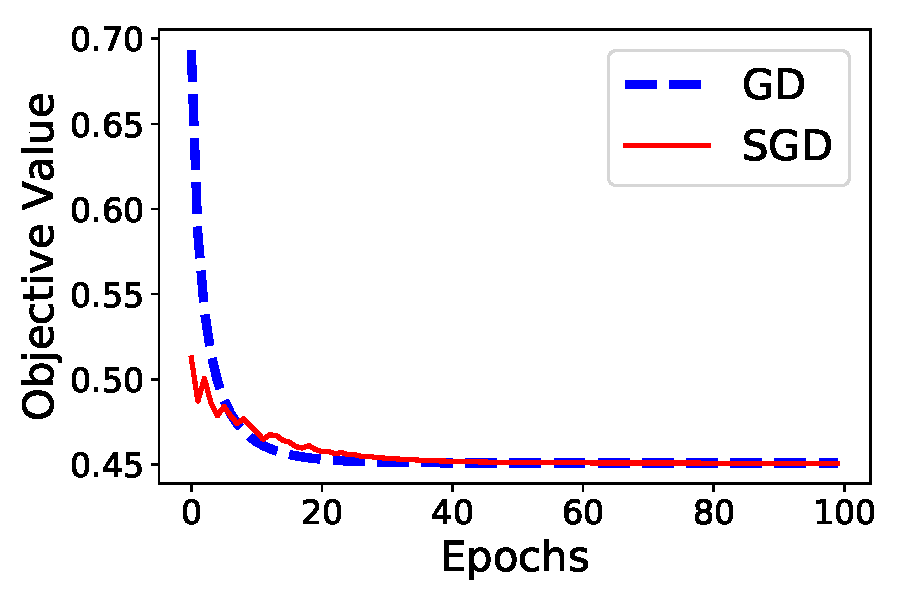
\includegraphics[width=0.6\linewidth]{figures/compare_gd_sgd.pdf}
	\caption{Plot of objective function value against epochs.
		SGD is tremendously faster than GD in the first 2 epochs,
		which means SGD can find a low-quality solution very efficiently.}
	\label{fig:compare_gd_sgd}
\end{figure}







\subsection{Definitions of terminologies} \label{sec:alg:terminologies}



\paragraph{Iteration.}
One iteration means performing one update of the variable $\w$.

\paragraph{Epoch.}
One epoch means every of the $n$ samples is visited exactly once by an algorithm.
For GD, one epoch is equivalent to one iteration.
For SGD, one epoch amounts to $n$ iterations.
For MB-SGD with batch size $b$, one epoch amounts to $\frac{n}{b}$ iterations.


\paragraph{Convergence.}
An algorithm is said to converge to $\w^\star$ 
if $\| \w_t - \w^\star \|$ is arbitrarily close to zero for a sufficiently large $T$ and all $t \geq T$


\paragraph{Warm-start.}
Initialize $\w$ using an estimate of $\w^\star$.
For example, with the regularization parameter $\lambda = 10^{-3}$, we obtain a solution $\tilde{\w}$;
then with a different setting, $\lambda = 10^{-6}$, we can use $\tilde{\w}$ as the initialization.



\paragraph{Strongly convex function.}
The function's graph is above a quadratic function.


\section{Making Predictions} \label{sec:predict}



By solving the logistic regression model \eqref{eq:model}, 
we can use the solution $\w \in \RB^d$ for making predictions.
For a test sample $\x' \in \RB^d$, we make prediction by
\begin{equation*}
f (\x')
\: = \: \sgn \big(  \w^T \x' \big) .
\end{equation*}

{\bf Classification accuracy or error rate} are the commonly used evaluation metrics.
For the class-balanced problems, that is, the numbers of postive samples and negative samples are comparable,
we can safely use classification accuracy or error rate.

However, for the {\bf class-imbalanced problems}, we shall never use such metrics.
For example, suppose we want to apply logistic regression to dectect phishing emails,
and $0.1\%$ among all the emails are phishing emails.
Then the classifier $f (\x') = -1$, which always makes non-phishing prediction disregarding the email content, will achieve a classification accuracy of $99.9\%$.
Such a classifier is obviously useless, although its classification accuracy is extremely high.
For class-imbalanced problems, we can use any of {\bf precision and recall}, {\bf F-measure}, {\bf receiver operating characteristic (ROC) curve}, or {\bf area under the curve (AUC)} as the evaluation metric.
Please refer to the Wikipedia pages for the definitions and examples.


\section{Cross-Validation}



In the logistic regression model \eqref{eq:model}, the optimization variable $\w$ is called {\it parameters} or {\it weights} in machine learning.
The parameters can be directly learned from the training data using numerical optimization.


\paragraph{Hyper-parameters.}
The other parameters, including the regularization parameter $\lambda$, learning rate $\alpha$, momentum parameter $\beta$, batch size $b$, and the number of epochs $T$, are called hyper-parameters.
Their setting determines the parameters $\w$, which is why they are called hyper-parameters.
\begin{itemize}
	\item 
	Hyper-parameters in the model.
	In the logistic regression model \eqref{eq:model},
	$\lambda$ is the only hyper-parameter,
	and the optimal $\w$ is a function of $\lambda$.
	\item
	Hyper-parameters in the optimization algorithm.
	The MB-SGD with momentum algorithm has 4 hyper-parameters:
	learning rate $\alpha$, momentum parameter $\beta$, batch size $b$, and the number of epochs $T$.
	Among them, $\alpha$, $\beta$, and $b$ affects the convergence rate and runtime, 
	while $T$ determines the closeness to the global minimum.
	For strongly convex models, the computed $\w$ may not depend on these hyper-parameters, especially when $T$ is sufficiently large.\footnote{For strongly convex models, the global minimum is unique, and the discussed algorithms all converge to the global minimum after sufficiently many epochs.
		However, for nonconvex models such as deep neural networks, the solution $\w$ is a function of all the four hyper-parameters: $\alpha$, $\beta$, $b$, and $T$; a small change of any of them will leads to a different solution $\w$.}
\end{itemize}
The hyper-parameters cannot be learned from the training data using numerical optimization.
How can we determine the hyper-parameters?




\paragraph{Cross-validation.}
If our goal is a low classification error rate on the test set, 
then an intuitively idea would be try all the possible combinations of hyper-parameters and adopt the combination which {\bf minimizes the test error}.
Unfortunately, this idea is very \textbf{wrong}.
All the model parameters and hyper-parameters must be independent of the test data; it would be otherwise cheating.
Keep in mind: Never use test data for hyper-parameter tuning!

The right approach to hyper-parameter tuning is {\bf cross-validation}.
Specifically, randomly partition the training data to two subset: one is training set, and the other is validation set.
Learn the model parameters on training set, 
and then evaluate the classification error on the validation set;
the error is called validation error.
You can try different combinations of hyper-parameters and choose the combination which minimizes the validation error.



The simple idea works in practice.
More often than not, the chosen combination of hyper-parameters may not be the ``best''.
Due to the randomness in the partition, the combination may happen to be the best for this specific partition;
by doing another random partitioning, another combination will be selected.






\begin{figure}[!h]
	\centering
	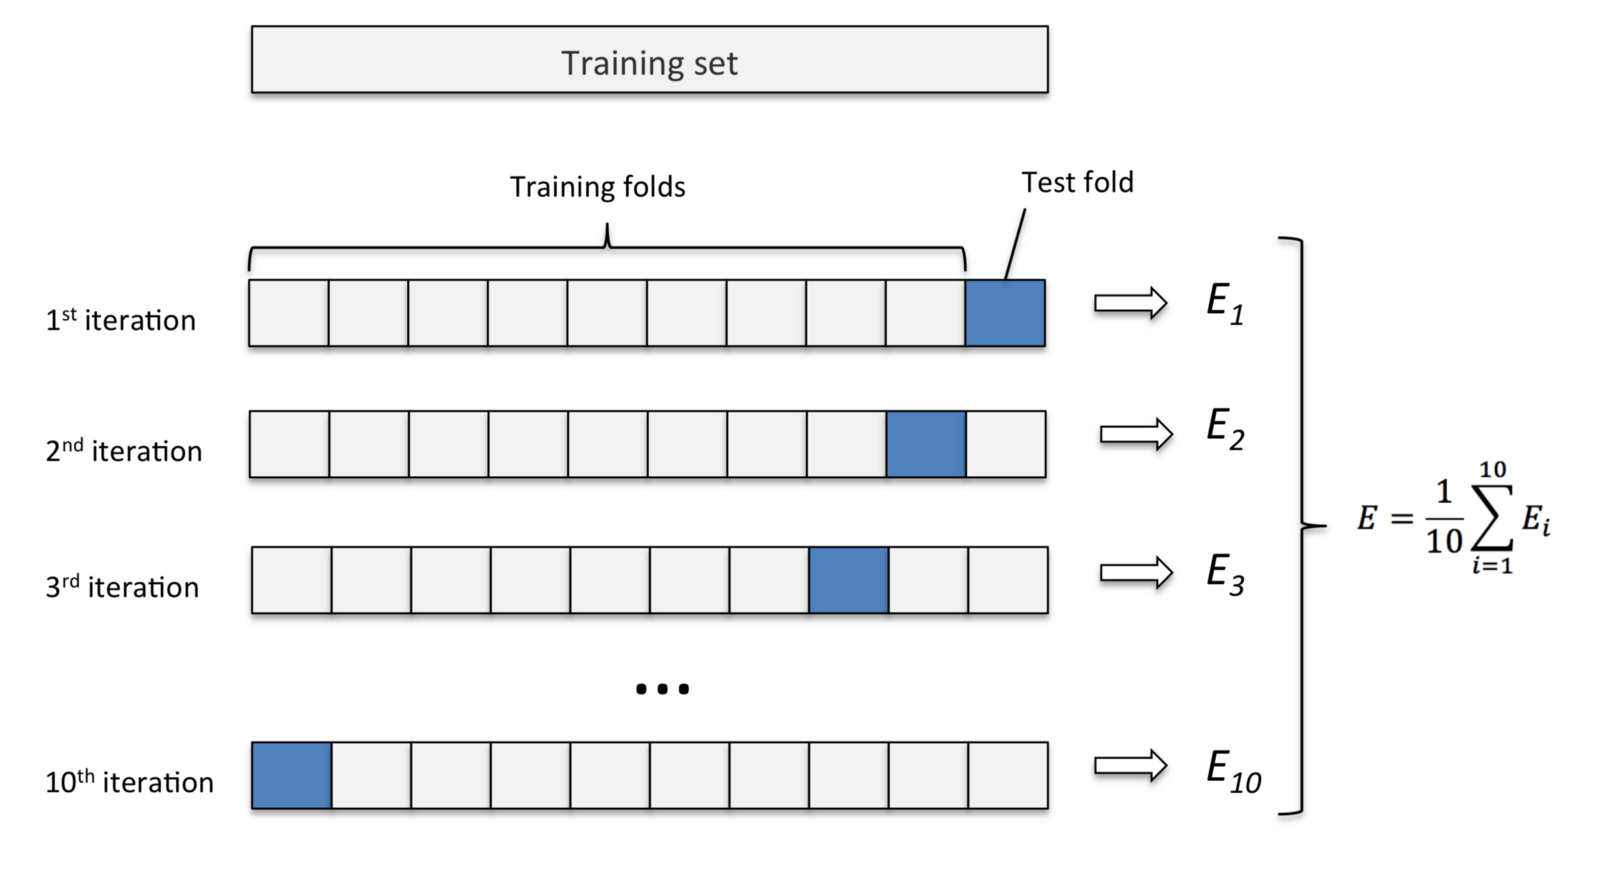
\includegraphics[width=0.8\linewidth]{figures/cv.png}
	\caption{Illustration of 10-fold cross-validation.
		The figure is from \url{http://karlrosaen.com/ml/learning-log/2016-06-20/}.}
	\label{fig:cv}
\end{figure}

\paragraph{$k$-fold cross-validation.}
A better idea is to repeat the random partition many times to reduce variance,
and it leads to the $k$-fold cross-validation.
Figure~\ref{fig:cv} illustrates the 10-fold cross-validation.
The training set is randomly partitioned to 10 subsets.
The model is trained using 9 subsets and validated on the remaining subset;
in this way, we get a validation error $E_1$.
By doing the same for the other partitions, we will get the validation errors $E_2, E_3, \cdots , E_{10}$
and the mean $E = \frac{1}{10} ( E_1 + \cdots + E_{10})$.
Notice that one combination of hyper-parameters leads to one validation error $E$;
we choose the combination that minimizes $E$.

Hyper-parameter tuning is computation intensive.
Using the $k$-fold cross-validation, we have to train the model for $k$ times, which leads to a significant increase in the computation.
In addition, there may be many combinations of hyper-parameters, especially when the model and algorithm have many hyper-parameters.
\textbf{If there are $c$ combinations of hyper-parameters and we use the $k$-fold cross-validation,
then we will have to solve the model for $ck$ times!}
Keep in mind, hyper-parameter tuning is the most time consuming step in machine learning.


\section{Problems}

\paragraph{P1.}
Implement mini-batch stochastic gradient descent (MB-SGD) by following the implementation of SGD.


\paragraph{P2.}
Implement MB-SGD with momentum by slightly modifying the code of MB-SGD.


\paragraph{P3.}
Compare MB-SGD and MB-SGD with momentum by plotting objective value against epochs as in Figure~\ref{fig:compare_gd_sgd}.

\paragraph{P4.}
The $d$-dim vector $\frac{ \partial \, l_i }{\partial \, \w }$ is defined in \eqref{eq:grad1}.
Calculate the derivative of vector w.r.t.\ vector:
\begin{equation*}
\frac{ \partial  }{\partial \, \w } \bigg( \frac{ \partial \, l_i }{\partial \, \w } \bigg)
\: = \: \frac{ \partial  }{\partial \, \w }  \bigg( \frac{ - y_i \x_i }{1+\exp({y_i \w^T x_i})} \bigg) .
\end{equation*}
Notice that the result is a $d\times d$ matrix.

\paragraph{P5.}
The Hessian matrix is the second derivative of the objective function $Q (\w; \X, y)$ w.r.t.\ $\w$.
Please derive the Hessian matrix (which is $d\times d$):
\begin{equation*}
\nabla^2 Q (\w) 
\: \triangleq \: 
\frac{ \partial \, Q (\w; \X, \y) }{ \partial \, \w \, \partial \, \w^T }
\: = \:
\frac{1}{n} \sum_{i=1}^n 
\frac{ \partial  }{ \partial \, \w} \bigg(\frac{ \partial \, l_i }{ \partial \, \w} \bigg)
+ {\lambda} \cdot
\frac{ \partial \, \w }{ \partial \, \w} .
\end{equation*}



\paragraph{P6.}
For the regularized logistic regression model \eqref{eq:model}, 
$\lambda$ is the only hyper-parameter needs fine tuning.\footnote{If you use MB-SGD with momentum, a rough setting of the hyper-parameters $\alpha$, $\beta$, $b$, and $T$, will work well.}
Implement 5-fold cross-validation to find out the ``best'' $\lambda$.\\
Hint: Select $\lambda$ from a set such as $\{ 10^{-10}, 10^{-9}, \cdots, 10^{0}, 10^1, 10^2 \}$ to minimize the validation error $E = \frac{1}{5} (E_1 + \cdots + E_5)$.



%\vspace{3mm}
%\begin{lstlisting}
%import numpy
%
%def rfm(x, s, sigma):
%	n, d = x.shape
%	a = numpy.random.standard_normal((d, s)) / sigma
%	b = numpy.random.rand(1, s) * (2 * numpy.pi)
%	c = numpy.dot(x, a) + b
%	h = numpy.cos(c) * numpy.sqrt(2/s)
%	return h
%\end{lstlisting}
%\vspace{3mm}

%\newpage
%\bibliographystyle{plain}
%
%%\markboth{\bibname}{\bibname}
%\bibliography{matrix}


\end{document}
